% !TEX TS-program = pdflatexmk
\documentclass[12pt]{article}

% Layout.
\usepackage[top=1in, bottom=0.75in, left=1in, right=1in, headheight=1in, headsep=6pt]{geometry}

% Fonts.
\usepackage{mathptmx}
\usepackage[scaled=0.86]{helvet}
\renewcommand{\emph}[1]{\textsf{\textbf{#1}}}
\newcommand{\ans}[1][1in]{\rule{#1}{.5pt}}

\usepackage[parfill]{parskip}

% Misc packages.
\usepackage{amsmath,amssymb,latexsym}
\usepackage{graphicx,hyperref}
\usepackage{array}
\usepackage{xcolor}
\usepackage{multicol,tikz}
\usepackage{tabularx,colortbl,booktabs,xparse}
\usepackage{enumitem}

% Rotation: \rot[<angle>][<width>]{<stuff>}
\NewDocumentCommand{\rot}{O{45} O{1em} m}{\makebox[#2][l]{\rotatebox{#1}{#3}}}%

\usepackage{fancyhdr}
\pagestyle{fancy} 
\lhead{\large\sf\textbf{MATH F113X: Kruskal's Algorithm}}
%\chead{\large\sf\textbf{lecture notes}}
%\rhead{\large\sf\textbf{Day 1}}

\begin{document}

Goals:
\begin{itemize}
\item Understand the terms: tree, spanning tree, minimum cost spanning tree
\item Understand how to use Kruskal's Algorithm to find a minimum cost spanning tree
\item Know of applications of minimum cost spanning trees
\end{itemize}
\begin{enumerate}
\item Definitions
	\begin{enumerate}
	\item \textbf{(tree)}
	\vfill
	\item \textbf{(spanning tree)}
	\vfill
	\item \textbf{(minimum cost spanning tree)}
	\vfill
	\end{enumerate}
\item Example: \\
\fbox{
\begin{minipage}{.5\linewidth}
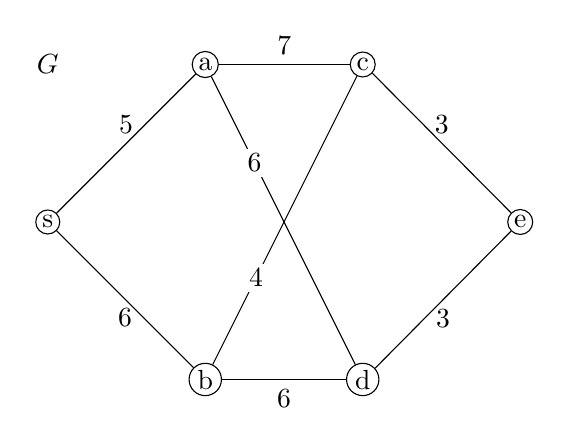
\begin{tikzpicture}[scale=2]
\node at (0,1){$G$};
\node[draw,circle, inner sep=1pt](s) at (0,0){s};
\node[draw,circle, inner sep=1pt](a) at (1,1){a};
\node[draw,circle, inner sep=1pt](b) at (1,-1){b};
\node[draw,circle, inner sep=1pt](c) at (2,1){c};
\node[draw,circle, inner sep=1pt](d) at (2,-1){d};
\node[draw,circle, inner sep=1pt](e) at (3,0){e};
\draw (s) -- (a) node [midway,above]{5};
\draw (s) -- (b) node [midway,below]{6};
\draw (a) -- (c) node [midway,above]{7};
\draw (a) -- (d) node [pos = .3, inner sep = 2pt, fill = white]{6};
\draw (b) -- (c) node [pos = .3, inner sep = 2pt, fill = white]{4};
\draw (b) -- (d) node [midway,below]{6};
\draw (d) -- (e) node [midway,below]{3};
\draw (c) -- (e) node [midway,above]{3};
\end{tikzpicture}
\end{minipage}
}

\newpage
\item
\fbox{Kruskal's Algorithm}

\textbf{input:} a graph, $G$, with costs (or weights) on the edges\\
\textbf{output:} a spanning tree, $T$, of minimum cost\\
\textbf{Steps:}
\begin{enumerate}
	\item (Initialization Step:) $T$ is a graph on the vertex set of $G$ but with no edges.
	\item (Iterative Step:) 
		\begin{enumerate}
		\item Select the cheapest unused edge in the graph. (Ties are broken alphabetically.)
		\item If the edge does \emph{not} create a cycle, add the edge to $T$. Otherwise, reject the edge.
		\item Mark the edge as used.
		\item If $T$ is a spanning tree, terminate the algorithm. Otherwise return to the beginning of the iterative step.
		\end{enumerate}
\end{enumerate}

\item Use Kruskal's Algorithm to find the minimum cost spanning tree for the graph $G$ below.

\vspace{1cm}
%%G%%
\fbox{
\begin{minipage}{.5\linewidth}
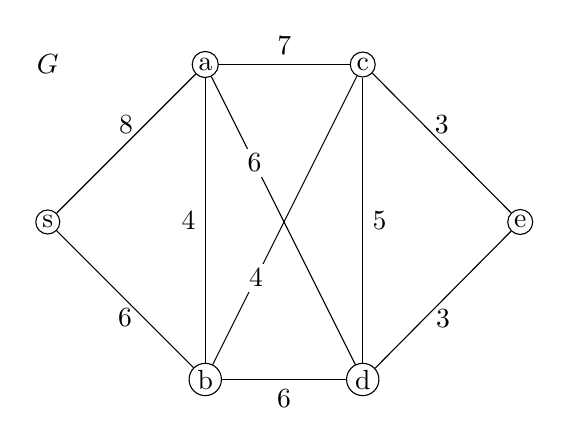
\begin{tikzpicture}[scale=2]
\node at (0,1){$G$};
\node[draw,circle, inner sep=1pt](s) at (0,0){s};
\node[draw,circle, inner sep=1pt](a) at (1,1){a};
\node[draw,circle, inner sep=1pt](b) at (1,-1){b};
\node[draw,circle, inner sep=1pt](c) at (2,1){c};
\node[draw,circle, inner sep=1pt](d) at (2,-1){d};
\node[draw,circle, inner sep=1pt](e) at (3,0){e};
\draw (s) -- (a) node [midway,above]{8};
\draw (s) -- (b) node [midway,below]{6};
\draw (a) -- (b) node [midway,left]{4};
\draw (a) -- (c) node [midway,above]{7};
\draw (a) -- (d) node [pos = .3, inner sep = 2pt, fill = white]{6};
\draw (b) -- (c) node [pos = .3, inner sep = 2pt, fill = white]{4};
\draw (b) -- (d) node [midway,below]{6};
\draw (d) -- (e) node [midway,below]{3};
\draw (c) -- (e) node [midway,above]{3};
\draw (c) -- (d) node [midway,right]{5};
\end{tikzpicture}
\end{minipage}
}
%%%%%%%
%%T%%
\fbox{
\begin{minipage}{.5\linewidth}
\begin{tikzpicture}[scale=2]
\node at (1,1.2){$\quad$};
\node at (1,-1.2){$\quad$};
\node at (0,1){$T$};
\node[draw,circle, inner sep=1pt](s) at (0,0){s};
\node[draw,circle, inner sep=1pt](a) at (1,1){a};
\node[draw,circle, inner sep=1pt](b) at (1,-1){b};
\node[draw,circle, inner sep=1pt](c) at (2,1){c};
\node[draw,circle, inner sep=1pt](d) at (2,-1){d};
\node[draw,circle, inner sep=1pt](e) at (3,0){e};
\end{tikzpicture}
\end{minipage}
}
%%%%%%%
\vfill
\begin{minipage}[t]{.5\linewidth}
\begin{tabular}{ c | p{2in} | p{2in}}
Used? &edges & weights\\ \hline
& \\
& \\
& \\& \\& \\& \\& \\& \\& \\% \\& \\& \\
 \end{tabular}
 \end{minipage}
 
 
\vfill
\item Think of an application of Kruskal's Algorithm.

\vfill
\end{enumerate}
\end{document}